\chapter{Existing ECS and Game Engines}\label{chap:existing}

In this chapter we will talk about the ECS concept, the history behind it and existing ECS libraries and game engines. This includes the first games that used a similar pattern to the now well known ECS architecture, as well as the people that established modern terminology around the ECS concept. We will also compare some existing ECS libraries and group existing game engines.

\section{ECS Concept}

\begin{figure}[h!]
\centering
\tikzstyle{box}=[rectangle,draw,rounded corners=0.5ex,minimum height=0.5cm,minimum width=1.5cm]
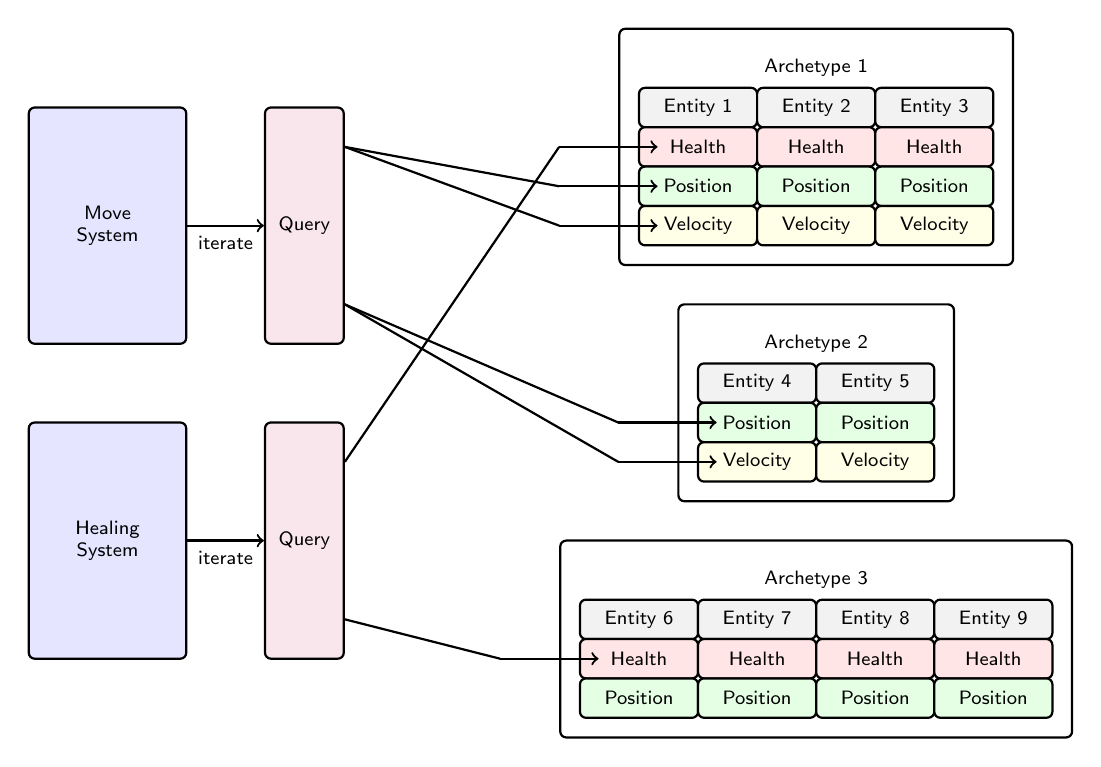
\begin{tikzpicture}[thick,font=\sf\scriptsize]
\node[box,minimum height=3cm,minimum width=5cm] at (0,0) {};
\node[] at (0,1) {Archetype 1};
\node[box,fill=gray!10] at (-1.5,0.5) {Entity 1};
\node[box,fill=gray!10] at (0,0.5) {Entity 2};
\node[box,fill=gray!10] at (1.5,0.5) {Entity 3};
\node[box,fill=red!10] (a1h) at (-1.5,0) {Health};
\node[box,fill=red!10] at (0,0) {Health};
\node[box,fill=red!10] at (1.5,0) {Health};
\node[box,fill=green!10] (a1p) at (-1.5,-0.5) {Position};
\node[box,fill=green!10] at (0,-0.5) {Position};
\node[box,fill=green!10] at (1.5,-0.5) {Position};
\node[box,fill=yellow!10] (a1v) at (-1.5,-1) {Velocity};
\node[box,fill=yellow!10] at (0,-1) {Velocity};
\node[box,fill=yellow!10] at (1.5,-1) {Velocity};

\node[box,minimum height=2.5cm,minimum width=3.5cm] at (0,-3.25) {};
\node[] at (0,-2.5) {Archetype 2};
\node[box,fill=gray!10] at (-0.75,-3) {Entity 4};
\node[box,fill=gray!10] at (0.75,-3) {Entity 5};
\node[box,fill=green!10] (a2p) at (-0.75,-3.5) {Position};
\node[box,fill=green!10] at (0.75,-3.5) {Position};
\node[box,fill=yellow!10] (a2v) at (-0.75,-4) {Velocity};
\node[box,fill=yellow!10] at (0.75,-4) {Velocity};

\node[box,minimum height=2.5cm,minimum width=6.5cm] at (0,-6.25) {};
\node[] at (0,-5.5) {Archetype 3};
\node[box,fill=gray!10] at (-2.25,-6) {Entity 6};
\node[box,fill=gray!10] at (-0.75,-6) {Entity 7};
\node[box,fill=gray!10] at (0.75,-6) {Entity 8};
\node[box,fill=gray!10] at (2.25,-6) {Entity 9};
\node[box,fill=red!10] (a3h) at (-2.25,-6.5) {Health};
\node[box,fill=red!10] at (-0.75,-6.5) {Health};
\node[box,fill=red!10] at (0.75,-6.5) {Health};
\node[box,fill=red!10] at (2.25,-6.5) {Health};
\node[box,fill=green!10] (a3p) at (-2.25,-7) {Position};
\node[box,fill=green!10] at (-0.75,-7) {Position};
\node[box,fill=green!10] at (0.75,-7) {Position};
\node[box,fill=green!10] at (2.25,-7) {Position};

\node[box,align=center,fill=blue!10,minimum height=3cm,minimum width=2cm] (gs) at (-9,-1) {Move\\System};
\node[box,align=center,fill=purple!10,minimum height=3cm,minimum width=1cm] (gsq) at (-6.5,-1) {Query};
\draw[->] (gs) -- node[midway,anchor=north] {iterate} (gsq);
\draw[-] ([yshift=1cm] gsq.east) -- ([xshift=-1cm] a1p.west);
\draw[->] ([xshift=-1cm] a1p.west) -- ([xshift=0.25cm] a1p.west);
\draw[-] ([yshift=1cm] gsq.east) -- ([xshift=-1cm] a1v.west);
\draw[->] ([xshift=-1cm] a1v.west) -- ([xshift=0.25cm] a1v.west);
\draw[-] ([yshift=-1cm] gsq.east) -- ([xshift=-1cm] a2p.west);
\draw[->] ([xshift=-1cm] a2p.west) -- ([xshift=0.25cm] a2p.west);
\draw[-] ([yshift=-1cm] gsq.east) -- ([xshift=-1cm] a2v.west);
\draw[->] ([xshift=-1cm] a2v.west) -- ([xshift=0.25cm] a2v.west);

\node[box,align=center,fill=blue!10,minimum height=3cm,minimum width=2cm] (ds) at (-9,-5) {Healing\\System};
\node[box,align=center,fill=purple!10,minimum height=3cm,minimum width=1cm] (dsq) at (-6.5,-5) {Query};
\draw[->] (ds) -- node[midway,anchor=north] {iterate} (dsq);
\draw[-] ([yshift=1cm] dsq.east) -- ([xshift=-1cm] a1h.west);
\draw[->] ([xshift=-1cm] a1h.west) -- ([xshift=0.25cm] a1h.west);
\draw[-] ([yshift=-1cm] dsq.east) -- ([xshift=-1cm] a3h.west);
\draw[->] ([xshift=-1cm] a3h.west) -- ([xshift=0.25cm] a3h.west);
\end{tikzpicture}
\caption{Example ECS structure (archetype based) with 3 archetypes and 2 systems. The \textit{Move System} queries and iterates over \textit{Position} and \textit{Velocity} components, the \textit{Healing System} over \textit{Health} components.}
\label{fig:ecs}
\end{figure}

The Entity Component System concept is not a single system, but rather an architectural pattern that is often used in game engines. It is based on the principle `composition over inheritance' and therefore uses a data-oriented design instead of an object-oriented design. It models a \textit{world} in terms of components, entities and systems.

\textit{Components} are a single piece of data, like a simple struct, for example a player's/NPC character's |Health| (Integer) or |Velocity| (2D or 3D Vector). \textit{Entities} are usually just an identifier or index, that identifies a single collection of these (different) components that work together to create that entity implicitly. For single instance data, like |Time| or |Assets|, some ECSs introduce \textit{Resources} that can be used inside a system besides component queries to hold a single value that does not belong to any entity. Other ECSs use a \textit{Singleton entity} concept for that, which ensures that such a global resource is added to one entity only.

\textit{Systems} are functions that transform components from one state to the next, acting on a \textit{Query} of components, independent of the purpose of the corresponding entities. These systems should not hold any data themselves, as they are only meant to define the code that transforms a set of components. Systems can then be run by the engine in their order every frame for single threaded applications. For efficient multithreading, the systems can be scheduled in parallel while avoiding any race conditions or modification during iteration. This can be done by making sure only one system has write access to a specific component type at the same time.

Many ECS libraries are \textit{archetype} based. Archetypes group entities by the set of components types they have, meaning multiple entities usually belong to the same archetype, which all have the same components with potentially different values. In the example presented in \Cref{fig:ecs}, \textsf{Archetype 1} could represent player entities with a |Health|, |Position| and |Velocity| component, whereas \textsf{Archetype 2} with |Position| and |Velocity| could represent any simple moving object, like bullets. \textsf{Archetype 3} could represent stationary enemies with just a |Health| and |Position|. The \textsf{Move System} iterates all entities with |Position| and |Velocity| to modify the entity's position based on its velocity, which would be all rigidbody physics objects. The \textsf{Healing System} just iterates over all |Health| components to increase the entity's health over time. This would heal players, as well as enemies, over time.

\section{ECS History}

A data-driven entity-based architecture with component databases for games was first implemented by the game \textsf{Thief: The Dark Project} (Looking Glass Studios, 1998)~\footnote{\url{https://thief.fandom.com/wiki/Thief:_The_Dark_Project}}~\footnote{\url{https://en.wikipedia.org/wiki/Thief:_The_Dark_Project}}. They had many financial problems during their development which shifted the focus of the game, but managed to release it working well. This was in part to their \textsf{Dark Object System}, which was the foundation for their \textsf{Dark Engine}~\footnote{\url{https://thief.fandom.com/wiki/Dark_Engine}}~\footnote{\url{https://en.wikipedia.org/wiki/Dark_Engine}}. The system is an ECS-like database for managing all the objects and assets in the world. It allowed game designers to modify and add/remove objects without changing code. This system worked so well, that they used it in their later game \textsf{System Shock 2} (1999), which for the most part even used the same executable of the engine.

After that, Scott Bilas from \textsf{Gas Powered Games} presented the approach they used for their \textsf{Dungeon Siege} game, with the title \textsf{A Data-Driven Game Object System} in 2002~\footnote{\url{https://www.gamedevs.org/uploads/data-driven-game-object-system.pdf}}. They needed a flexible system to manage over 7300 unique objects and over 100000 total objects in continuous, dynamically loaded maps. This should also work without engineers needing to modify and potentially hack/work around code, with the goal to empower designers to directly add objects and functionality to the world. For this problem, they also invented an object system, although it was quite different from modern ECS implementations. This presentation started to increase the attention around the ECS/data-driven architecture for games.

In 2007 Mick West from Neversoft also talked about their ECS in the article \textsf{Evolve Your Hierarchy}~\footnote{\url{https://cowboyprogramming.com/2007/01/05/evolve-your-heirachy/}}. It was further popularized by Adam Martin in his extensive blogposts starting in 2007, with the title \textsf{Entity Systems are the future of MMOG development}~\footnote{\url{https://t-machine.org/index.php/2007/09/03/entity-systems-are-the-future-of-mmog-development-part-1/}}. MMOG is the abbreviation of `Massive Multiplayer Online Game', referring to online games with many players, usually over 10 or 20 and sometimes even hundreds simultaneously. Adam Martin also established most of the modern terminology and concepts, like systems being first-class elements that actually hold (just) their code, components holding raw data and entities being just identifiers.

\section{Existing ECS Libraries}

The ECS architecture has been used in a wide range of applications, but mainly in the fields of games, simulations and other graphical/interactable media. One example is `Vico: An entity-component-system based co-simulation framework'~\cite{hatledal2021vico}. Others have improved parts of the concept, such as implementing wait-free hash maps for component access~\cite{lange2016wait}. Many more ECS libraries have been developed without written papers about them. Most of them are standalone for general purpose, but still intended for games and similar applications. There are so many ECS libraries, in fact, that we cannot go into details of comparing or grouping them, as that would be too much for the scope of this thesis. We will however go over some of the differences and data structures they use.

The first and one of the most important concepts is the memory layout of stored components. One approach is the \textit{archetype} concept, which our ECS uses as well. This means that any specific set of components an entity has at one time is called its archetype, which usually is dynamic. For dynamic approaches, any component can be added or removed from an entity at runtime, which makes it change archetypes dynamically. Examples of ECS libraries with archetypes include \textsf{flecs}~\footnote{\url{https://github.com/SanderMertens/flecs}}, \textsf{decs}~\footnote{\url{https://github.com/vblanco20-1/decs}}, \textsf{apecs} (by schell)~\footnote{\url{https://github.com/schell/apecs}}, \textsf{hecs}~\footnote{\url{https://github.com/Ralith/hecs}}, \textsf{legion}~\footnote{\url{https://github.com/amethyst/legion}} and the Unity DOTS ecs package~\footnote{\url{https://unity.com/ecs}}. Some of these ECS libraries combine that with a chunked approach, which splits the components of every archetype over multiple chunks, usually around 16 kB in size and memory alignment. This optimizes cache efficiency while not having to reallocate the whole array/vector when its current size limit is reached.

Another commonly used memory layout are \textit{sparse sets}, which in their core use two arrays/vectors; One is sparse and stores an index based on an item's directly, which then points to an index in the dense array/vector where the actual data is. This dense data array/vector has no empty indices and is therefore ideal for iteration, while the sparse one is used to locate or add/remove single components. This concept is used, for example, in the ECS libraries \textsf{shipyard}~\footnote{\url{https://github.com/leudz/shipyard}} and the well-known \textsf{EnTT}~\footnote{\url{https://github.com/skypjack/entt}}, which is used in the game \textsf{Minecraft (Bedrock)} (by Mojang)~\footnote{\url{https://www.minecraft.net}} among others. Other ECS libraries like \textsf{bevy\textunderscore ecs}~\footnote{\url{https://github.com/bevyengine/bevy/tree/main/crates/bevy_ecs}} from the \textsf{Bevy}~\footnote{\url{https://bevyengine.org/}} game engine use a hybrid approach, where in this case either a simple table layout can be used for fast iteration where all components of a type are stored in a single column, or a sparse set.

Other differences between the existing ECS libraries are mostly their API with the amount of boilerplate code needed and their additional features, that go beyond the very basic and essential core of an ECS. Boilerplate code in these cases is mostly having complex structures for the ECS parts that need to be initialized, having to implement specific traits to make a struct work as a component or requiring unnecissary long type signatures to be written out. Other boilerplate code includes needing to manual initialize different parts of the ECS, like registering a component type or how queries are used and when systems are executed. Some require more boilerplate code to use, but can be more idiomatic for the language and potentially easier to understand and work with in large projects. Others are based on the principle to make it as easy and simple to use with the least code possible. Additional features many of the existing libraries provide include systems instead of using queries explicitly and (multithreaded) scheduling for systems. Some also have change detection to filter components that might need to be processed again, as well as relations/relationships that can build the basis for parent/child hierarchies and other relations. A few libraries also include events and triggers/observers to avoid iterating many entities when only sometimes a single event is fired that needs the entities to be processed again.

\section{Grouping Existing Game Engines}

There are very view game engines that are developed with a focus on research or backed by freely available research papers that go over the full engine/architecture. This is why we have to compare community driven and commercial game engines without proper research focus as well.

\begin{table}[h!]
\centering
\begin{tabular}{p{4cm}p{4cm}p{4cm}}
\hline
\textbf{Group} & \textbf{Engines} & \textbf{Core Architecture} \\
\hline
Data-Oriented ECS &
Bevy, Unity (DOTS) &
Decouples data and behavior via components and systems \\
\hline
Object-Oriented Scene Graphs &
Unity (without DOTS), Unreal, Godot, PyGame, Löve, Three.js, Babylon.js &
Behavior via components/methods, often imperative update loops \\
\hline
Functional or Declarative Architectures &
Elm Game Engine, play-cljs, raylib in Haskell &
Pure state transformations and signals \\
\hline
\end{tabular}
\caption{Grouping game engines by architectural pattern.}
\label{tab:grouping}
\end{table}

The \Cref{tab:grouping} shows some of the existing game engines and splits them by their core architecture. The ECS architecture was already explained; it completely separates persistent data and behavior. The object-oriented pattern, mostly using some kind of scene graph, uses typical objects (classes/structs) with included behavior for its scene graph objects. These are sometimes combined to create a single game object, which also makes the system more composable instead of using inheritance, like in the Unity game engine. Functional and declarative architectures are much less common in game development. They define the game loop in a functional way, often declaratively defining the game objects/data. The transformations of the world are then (in the ideal case) purely functional.

Having examined a range of existing engine architectures, it becomes clear that while ECS and object-oriented patterns each offer modularity and performance in different ways, they do not easily support the composable, scoped, and expressive behavior abstraction that effects and handlers can provide. This motivates the design of our own engine implementation in Effekt, which explores combining effect systems with the ECS architecture for a simpler implementation and ergonomic interface, while still having the modularity and composability of the ECS architecture.
